% System architecture of the proposed system (Section 3).
% Standalone file: compile it on its own to get architecture.pdf (already included),
% or upload architecture.pdf to Overleaf and use \includegraphics.
\documentclass[tikz,border=4pt]{standalone}
\usepackage[T1]{fontenc}
\usepackage{lmodern}
\usetikzlibrary{positioning,arrows.meta,fit,backgrounds,calc}

% Colour-blind-safe palette (Okabe-Ito)
\definecolor{trainable}{HTML}{E69F00}   % orange: parameters updated by training
\definecolor{frozenc}{HTML}{999999}     % grey: frozen weights / no parameters
\definecolor{selectc}{HTML}{0072B2}     % blue: settings chosen without the test word
\definecolor{datac}{HTML}{56B4E9}       % light blue: data

\begin{document}
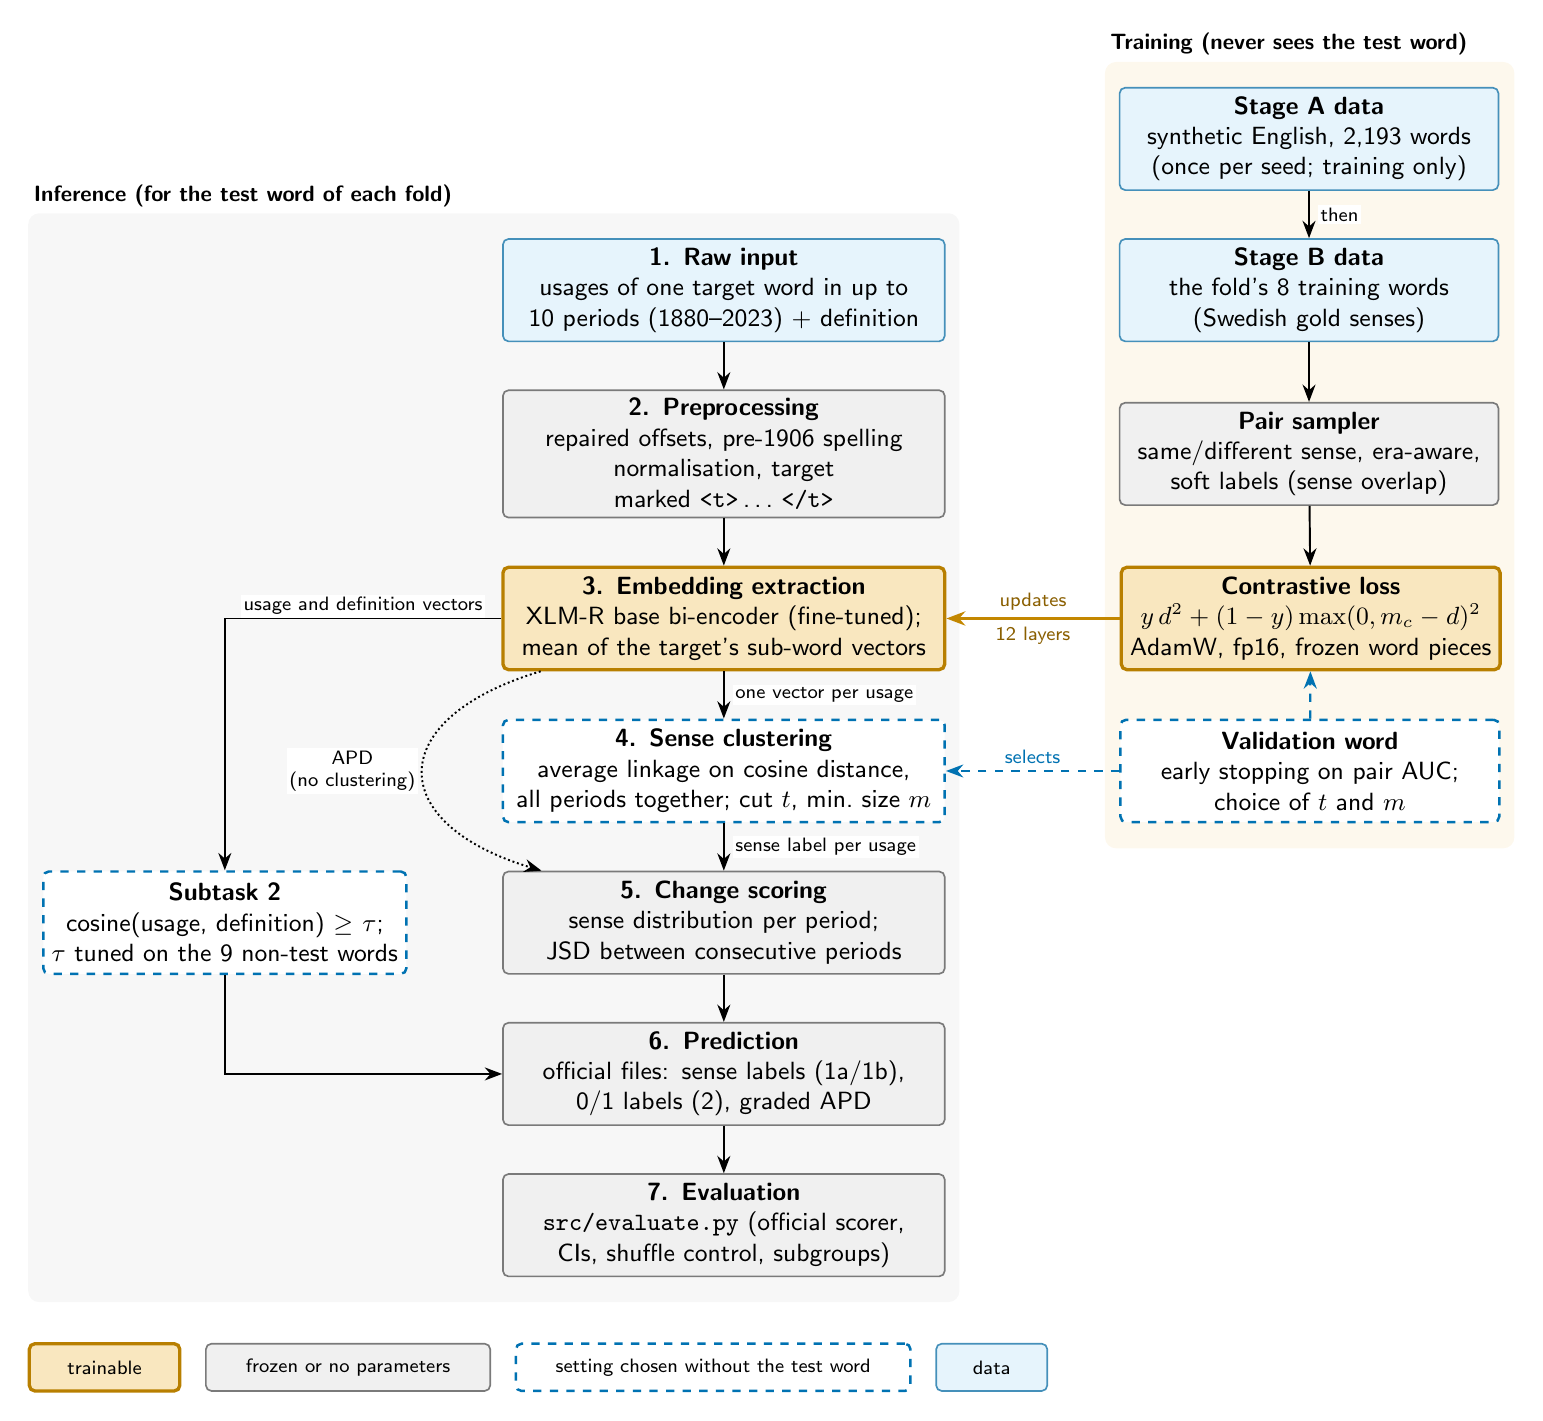
\begin{tikzpicture}[
  font=\sffamily\small,
  box/.style={draw, rounded corners=2pt, align=center, minimum height=13mm,
              text width=54mm, inner sep=3pt, line width=0.6pt,
              execute at begin node={\hyphenpenalty=10000\exhyphenpenalty=10000}},
  data/.style={box, fill=datac!15, draw=datac!80!black},
  frozen/.style={box, fill=frozenc!15, draw=frozenc!80!black},
  train/.style={box, fill=trainable!25, draw=trainable!80!black, line width=1.2pt},
  sel/.style={box, fill=white, draw=selectc, dashed, line width=0.9pt},
  arr/.style={-{Stealth[length=2.2mm]}, line width=0.7pt},
  tarr/.style={-{Stealth[length=2.4mm]}, line width=1.1pt, draw=trainable!85!black},
  sarr/.style={-{Stealth[length=2.2mm]}, line width=0.8pt, draw=selectc, dashed},
  lab/.style={font=\sffamily\scriptsize, align=center, fill=white, inner sep=1pt},
]
\def\vgap{6mm}

% ---------------- inference pipeline (centre column) ----------------
\node[data] (raw) {\textbf{1. Raw input}\\usages of one target word in up to\\10 periods (1880--2023) + definition};
\node[frozen, below=\vgap of raw] (pre) {\textbf{2. Preprocessing}\\repaired offsets, pre-1906 spelling\\normalisation, target marked \texttt{<t>}\,\dots\,\texttt{</t>}};
\node[train, below=\vgap of pre] (enc) {\textbf{3. Embedding extraction}\\XLM-R base bi-encoder (fine-tuned);\\mean of the target's sub-word vectors};
\node[sel, below=\vgap of enc] (clu) {\textbf{4. Sense clustering}\\average linkage on cosine distance,\\all periods together; cut $t$, min.\ size $m$};
\node[frozen, below=\vgap of clu] (chg) {\textbf{5. Change scoring}\\sense distribution per period;\\JSD between consecutive periods};
\node[frozen, below=\vgap of chg] (pred) {\textbf{6. Prediction}\\official files: sense labels (1a/1b),\\0/1 labels (2), graded APD};
\node[frozen, below=\vgap of pred] (eval) {\textbf{7. Evaluation}\\\texttt{src/evaluate.py} (official scorer,\\CIs, shuffle control, subgroups)};

\draw[arr] (raw) -- (pre);
\draw[arr] (pre) -- (enc);
\draw[arr] (enc) -- node[lab, right=1mm] {one vector per usage} (clu);
\draw[arr] (clu) -- node[lab, right=1mm] {sense label per usage} (chg);
\draw[arr] (chg) -- (pred);
\draw[arr] (pred) -- (eval);

% APD: graded change straight from the vectors (no clustering)
\draw[arr, densely dotted] ([xshift=5mm]enc.south west) .. controls +(-20mm,-6mm) and +(-20mm,6mm) ..
   node[lab, left=0.5mm, pos=0.5] {APD\\(no clustering)} ([xshift=5mm]chg.north west);

% ---------------- Subtask 2 (left column) ----------------
\node[sel, text width=44mm, left=12mm of chg] (s2) {\textbf{Subtask 2}\\cosine(usage, definition) $\geq\tau$;\\$\tau$ tuned on the 9 non-test words};
\draw[arr] (enc.west) -| node[lab, pos=0.25, above] {usage and definition vectors} (s2.north);
\draw[arr] (s2.south) |- (pred.west);

% ---------------- training (right column, aligned with the pipeline rows) ----------------
\node[data, text width=46mm, right=22mm of raw] (sv) {\textbf{Stage B data}\\the fold's 8 training words\\(Swedish gold senses)};
\node[data, text width=46mm, above=\vgap of sv] (syn) {\textbf{Stage A data}\\synthetic English, 2{,}193 words\\(once per seed; training only)};
\node[frozen, text width=46mm, right=22mm of pre] (pairs) {\textbf{Pair sampler}\\same/different sense, era-aware,\\soft labels (sense overlap)};
\node[train, text width=46mm, right=22mm of enc] (loss) {\textbf{Contrastive loss}\\$y\,d^2 + (1-y)\max(0, m_c-d)^2$\\AdamW, fp16, frozen word pieces};
\node[sel, text width=46mm, right=22mm of clu] (val) {\textbf{Validation word}\\early stopping on pair AUC;\\choice of $t$ and $m$};

\draw[arr] (syn) -- node[lab, right=1mm] {then} (sv);
\draw[arr] (sv) -- (pairs);
\draw[arr] (pairs) -- (loss);
\draw[tarr] (loss) -- node[lab, above=0.5mm, text=trainable!60!black] {updates} node[lab, below=0.5mm, text=trainable!60!black] {12 layers} (enc);
\draw[sarr] (val) -- node[lab, above=0.5mm, text=selectc] {selects} (clu);
\draw[sarr] (val) -- (loss);

% ---------------- panels ----------------
\begin{scope}[on background layer]
  \node[fit=(raw)(eval)(s2), fill=black!3, rounded corners=4pt, inner xsep=5pt, inner ysep=9pt,
        label={[font=\sffamily\footnotesize\bfseries, anchor=south west, inner sep=2pt]north west:Inference (for the test word of each fold)}] (pin) {};
  \node[fit=(syn)(val), fill=trainable!7, rounded corners=4pt, inner xsep=5pt, inner ysep=9pt,
        label={[font=\sffamily\footnotesize\bfseries, anchor=south west, inner sep=2pt]north west:Training (never sees the test word)}] (ptr) {};
\end{scope}

% ---------------- legend ----------------
\node[train, minimum height=6mm, text width=17mm, font=\sffamily\scriptsize, anchor=north west]
   (l1) at ([yshift=-5mm]pin.south west) {trainable};
\node[frozen, minimum height=6mm, text width=34mm, right=3mm of l1, font=\sffamily\scriptsize] (l2) {frozen or no parameters};
\node[sel, minimum height=6mm, text width=48mm, right=3mm of l2, font=\sffamily\scriptsize] (l3) {setting chosen without the test word};
\node[data, minimum height=6mm, text width=12mm, right=3mm of l3, font=\sffamily\scriptsize] (l4) {data};
\end{tikzpicture}
\end{document}
